The processor architecture is a MIPS-inspired pipelined architecture with five stages.
The five stages are called Instruction Fetch, Instruction Decode, Execution, Memory and Write Back.
Each stage is separated by pipeline registers that hold the relevant data for the different stages between clock cycles.
Since the the CPU is pipelined, it can achieve much higher performance than the simple multi-cycle processor architecture designed in the previous assignment\cite{assignment-1}.
For ideal execution, every component of the processor is in use in every cycle, giving a high utilization of resources.
Paradoxically, even though pipelined processor designs can be much more performant than simple multi-cycle processor designs, they are not necessarily more complex.
This is because there is no longer need for a massive state machine in the control unit in the pipeline processor, as there would be in a multi-cycle processor control unit.

Not everything is better with a pipelined design, however.
With a pipelined design, the processor is vulnerable to data hazards and control hazards.
A hazard, in processor design terminology, is a situation where a planned execution in a processor cannot be performed because it is dependant on the outcome of a previous execution which has not yet completed.
This is made possible because of the introduction of instruction-level parallelism.
The solution processor presented in this report resolves hazards by using a combination of data forwarding and stalling.
One type of hazard, the use-after-load\cn hazard, where an instruction relies on the data from a memory load in the instruction immediately preceeding it, is not handled by the processor.
Trying to execute an instruction which uses the result from a load immediately after the load instruction results in undefined behaviour.
Instead of handling this in hardware, the bundled solution assembler solves this issue by instruction reordering, or simply inserting nops where needed.
This is done to remove complexity from the processor core, which in turn increases processor performance, which is aligned with the performance goal from section \vref{subsection:performance}.

The processor architecture is modeled after the Harvard Architecture design, which means that it has separate instruction and data memory.
This, in addition to being a security boon, makes for a more performant design, as the instruction memory and data can be accessed independantly.
This is aligned with the performance design goal from \vref{subsection:performance}.

Having separate memories for data and instructions also removes the need for a central memory access arbitrage unit, which increases the simplicty of the design in accordance to the design goal in section\vref{subsection:simplicity}.

The processor architecture can bee seen illustrated in figure \vref{figure:architecture}.
The tall orange bars are the pipeline registers.
The blue lines are control signals.

\begin{figure}[H]
    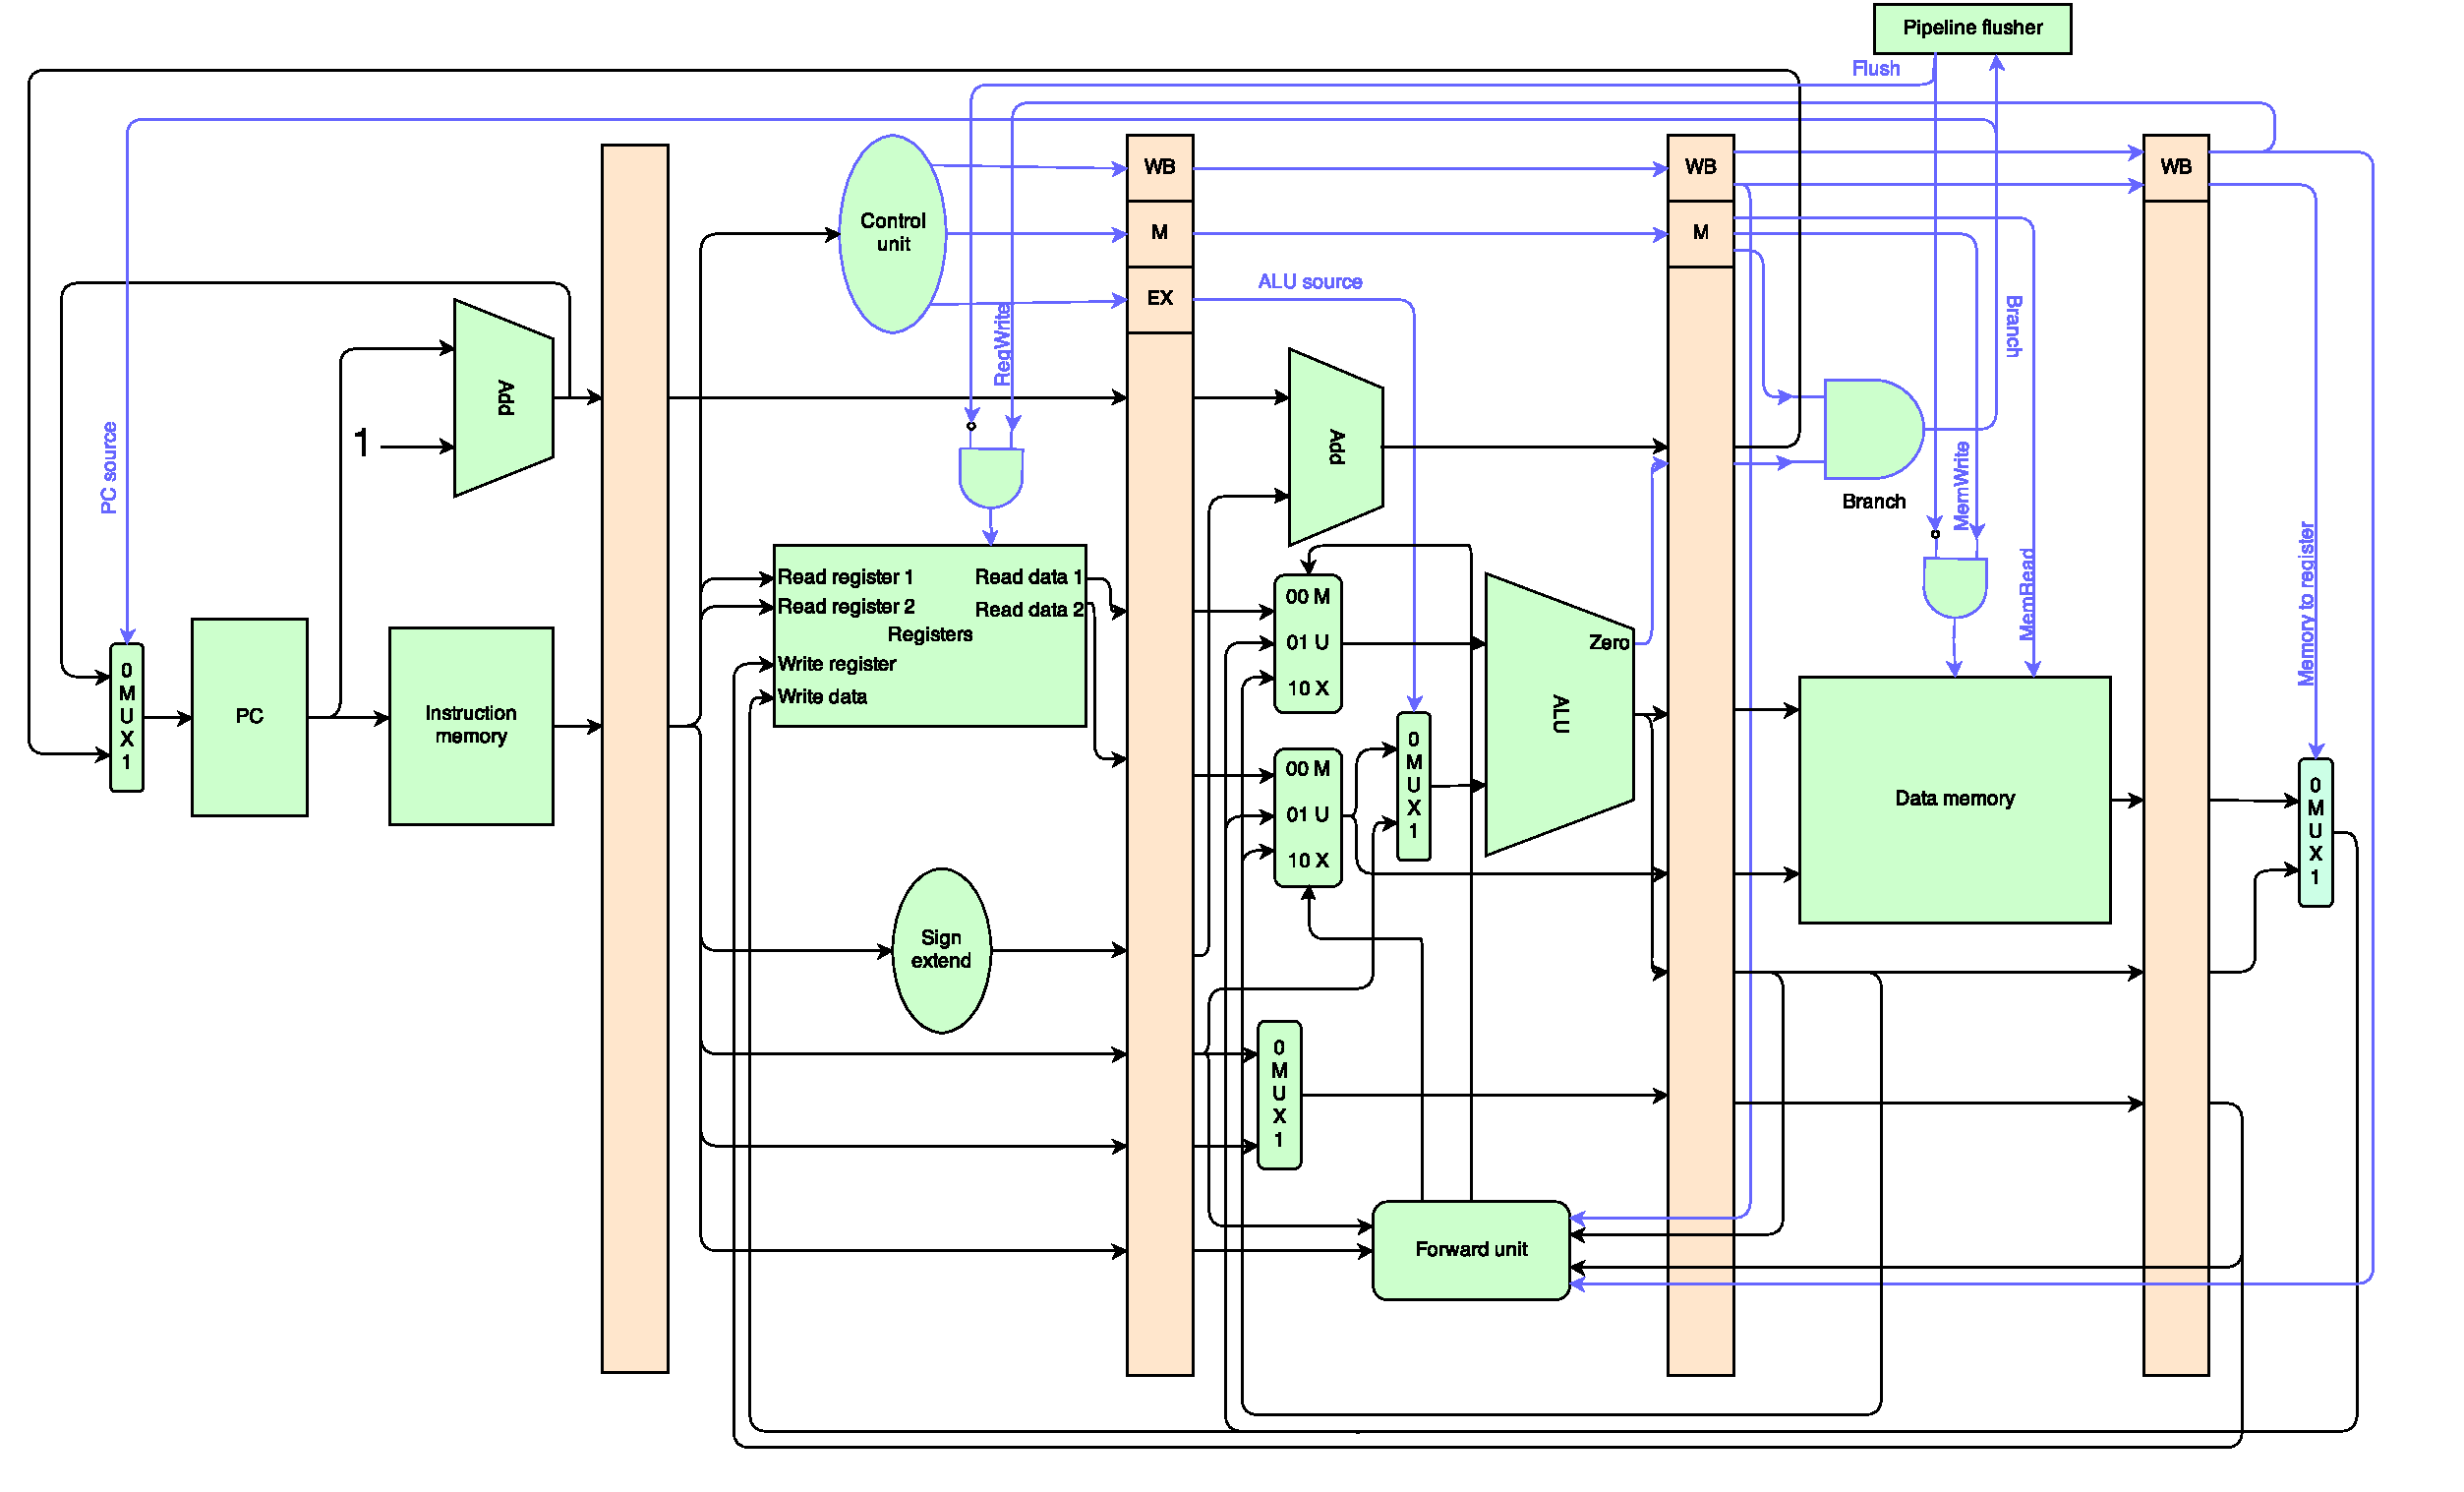
\includegraphics[width=\textwidth]{illustrations/processor.pdf}
    \caption{The processor architecture}
    \label{figure:architecture}
\end{figure}


The rest of this section describes the different architectural subcomponents in detail.

\subsection{Instruction Fetch Stage}
    The instruction fetch stage is the first stage in the processor pipeline.
It is responsible for fetching the correct instruction from the instruction memory, and feeding it to the next stage in the pipeline.

\subsubsection{Program Counter}
In order to know where in the program the processor is currently executing, a program counter is needed.
The program counter is a simple register which holds the instruction address of the address currently being fetched and sent on to the next stage in the pipeline.
The instruction fetch stage updates the program counter each cycle, either by increasing it by one so as to fetch the next instruction, or by to a different number requested by a different part of the processor, in the case of a jump.



\subsection{Instruction Decode Stage}
    \todo{picture of decode stage}

The instruction decode stage receives an instruction from the instruction fetch stage and understands it.
Using this understanding, it orchestrates and coordinates the execution of the instruction.
This means that it is responsible for preparing the necessary data for the ALU, and setting the appropriate control signals for the rest of the processor for each instruction.
The register file of the processor resides in the instruction decode stage, and register data that are needed in computation in the execution stage are fetched and prepared in the instruction decode stage.
The control unit also resides in this stage.

\newpage
\subsubsection{Register File}
    The register file is a large block of 32 registers that make up the general purpose registers of the processor that are accessible to users.
The register file implementation is the same as in the prevous assignment\cite{assignment-1}, and is also part of the supplied support files for this assignment.


\newpage
\subsubsection{Control Unit}
    The control unit is the component that is responsible for enabling and disabling the correct parts of the processor at the correct times, so that an instruction is executed correctly.

\subsubsection{In Signals}

\begin{description}
\item{\textbf{Instruction Op-code}} \\
    The op-code of the currently executing instruction in the instruction decode stage.

\item{\textbf{Instruction Function}} \\
    The ALU function of the currently executing instruction in the instruction decode stage. 
\end{description}

\subsubsection{Out Signals}

\begin{description}
\item{\textbf{Execute Control Signals}} \\
    The control signals that should be used in the execute stage for the instruction being decoded by the control unit.
    The execute control signals bus contains the \textbf{ALU Source}, \textbf{ALU Function} and \textbf{Register Destination} control signals.

\item{\textbf{Memory Control Signals}} \\
    The control signals that should be used in the memory stage for the instruction being decoded by the control unit.
    The memory control signals bus contains the \textbf{Branch} and \textbf{Memory Write} control signals.

\item{\textbf{Write-Back Control Signals}} \\
    The control signals that should be used in the write-back stage for the instruction being decoded by the control unit.
The write-back control signals bus contains the \textbf{Memory to Register} and \textbf{Register Write} control signals.

\item{\textbf{Jump}} \\
    Whether or not the instruction being decoded is a jumping instruction (i.e. \texttt{JMP}).
\end{description}




\subsection{Execution Stage}
    \todo{describe this stage}
\todo{image of this stage}

\subsubsection{ALU}
    \todo{The ALU description}

\subsubsection{In Signals}

\begin{description}
\item{\textbf{Signal}} \\
Description of it.

\end{description}

\subsubsection{Out Signals}

\begin{description}
\item{\textbf{Signal}} \\
Description of it.
\end{description}


\subsubsection{Forwarding Unit}
    The forwarding unit is responsible for forwarding newly computed data from later stages in the pipeline to earlier stages, where new instructions might need the data before they are commited to registers at the end of the pipeline.
The forwarding unit is essential to achieving a high performance pipelined design, as without it computations would either be wrong or slow.

The forwarding unit looks at which data is needed in the execution stage, and if the needed data has been updated down the pipeline but not in the register file, forwards the data to the ALU instead of the old data fetched from the register file by the instruction decode stage.
To be able to do this, the forwarding unit needs data from many different stages at once.

\subsubsection{In Signals}

\begin{description}
\item{\textbf{rs\_address\_from\_id\_ex}} \\
    The source register address of the Rs operand from the ID/EX pipeline registers.

\item{\textbf{rt\_address\_from\_id\_ex}} \\
    The source register address of the Rs operand from the ID/EX pipeline registers.

\item{\textbf{register\_destination\_from\_ex\_mem}} \\
    The destination register address from the EX/MEM pipeline registers.

\item{\textbf{register\_destination\_from\_mem\_wb}} \\
    The destination register address from the MEM/WB pipeline registers.

\item{\textbf{register\_write\_from\_ex\_mem}} \\
    The register write control signal from the EX/MEM pipeline registers.

\item{\textbf{register\_write\_from\_mem\_wb}} \\
    The register write control signal from the MEM/WB pipeline registers.
\end{description}

\subsubsection{Out Signals}

\begin{description}
\item{\textbf{forward\_rs\_out}} \\
    The forwarded value of the Rs register.

\item{\textbf{forward\_rt\_out}} \\
    The forwarded value of the Rt register.

\end{description}


\subsubsection{Hazard Detector}
    \todo{The Hazard Detector description}

\subsubsection{In Signals}

\begin{description}
\item{\textbf{register\_address\_in}} \\
Description of it.
\item{\textbf{register\_write\_execute\_in}} \\
Description of it.
\item{\textbf{register\_write\_memory\_in}} \\
Description of it.
\item{\textbf{register\_destination\_execute\_in}} \\
Description of it.
\item{\textbf{register\_destination\_memory\_in}} \\
Description of it.
\end{description}

\subsubsection{Out Signals}

\begin{description}
\item{\textbf{hazard\_out}} \\
Description of it.
\end{description}



\subsection{Memory Stage}
    \subsubsection{Data Memory}


\subsection{Write-Back Stage}
    The Write Back stage is responsible for routing the correct data to the register file, when data should be written to the register file.


\subsection{Additional Components}
    \subsubsection{Pipeline Registers}

Between each stage of the pipeline there are series of registers that hold the necessary values between clock ticks.
The pipeline registers are clocked synchronously, which means that the pipeline design is a buffered synchronous design.
The pipeline registers are implemented as flip-flops.


\subsubsection{Flip Flop}

A flip-flop is a simple circuit that has two stable states.
The implication is that they can be used to store values over time.

In the solution processor, size-generic flip-flops VHDL are used.
Because type generics were first introduced in the VHDL 2008 standard\cite{vhdl2008}, and the Xilinx tool chain doesn't support it yet, flip-flops are implemented on a per-type basis.
Subsequently, the \texttt{flip\_flop.vhd} VHDL source code file is a lot bigger and hairier than it could be.

\subsubsection{Multiplexers}

A multiplexer is a component which selects between multiple input signals based on a separate control signal.
Since multiplexers are use quite commonly, and VHDL has no build in construct for it, some multiplexer components are introduced in the solution.

\subsubsubsection{Multiplexer 2}

The Multiplexer 2 selects one of two possible input values based on the value of a 1-bit selection signal.

\subsubsubsection{Multiplexer 3}

The Multiplexer 3 selects one of three possible input values based on the value of a 2-bit selection signal.
Since a 2-bit selection signal may have 4 possible states, and the Multiplexer 3 only has three inputs, one of the selection signal states ("\texttt{11}") holds undefined behaviour.

\subsubsection{Pipeline flusher}

The pipeline flusher is reponsible for flushing the pipeline if a branch prediction goes wrong.
In such a case, the pipeline will be filled with instructions that shouldn't be executed.
The pipeline flusher disables these instructions by removing their ability to write to registers and memory.

